% vim: set textwidth=78 autoindent:

% when the revision of a section has been finalized,
% comment out the following line:
%\updatedisclaimer

\section{Spatial Analysis (Interpolation)}\label{sec:interpolation}
\begin{tabular}{p{3.5cm}p{6cm}p{6cm}}
\multirow{2}{*}{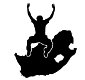
\includegraphics[width=2.5cm]{logo}} & Objectives: &
Understanding of interpolation as part of spatial analysis. \\
& & \\
& Keywords: & 
Point data, interpolation method, Inverse Distance Weighted, Triangulated
Irregular Network  \\
\hline
\end{tabular}

\subsection{Overview}

\textbf{Spatial analysis} is the process of manipulating spatial information
to extract
new information and meaning from the original data. Usually spatial analysis
is carried out with a Geographic Information System (GIS). A GIS usually
provides spatial analysis tools for calculating feature statistics and
carrying out  geoprocessing activities as data interpolation. 
In hydrology, users will likely emphasize the importance of terrain analysis
and hydrological modelling (modelling the movement of water over and in the
earth). In wildlife management, users are interested in analytical functions
dealing with wildlife point locations and their relationship to the
environment. Each user will have different things they are interested in
depending on the kind of work they do.

\subsection{Spatial interpolation in detail}

\begin{figure}[ht]
   \begin{center}
   \caption{Temperature map interpolated from South African Weather Stations.}
\label{fig:temperature}\smallskip
   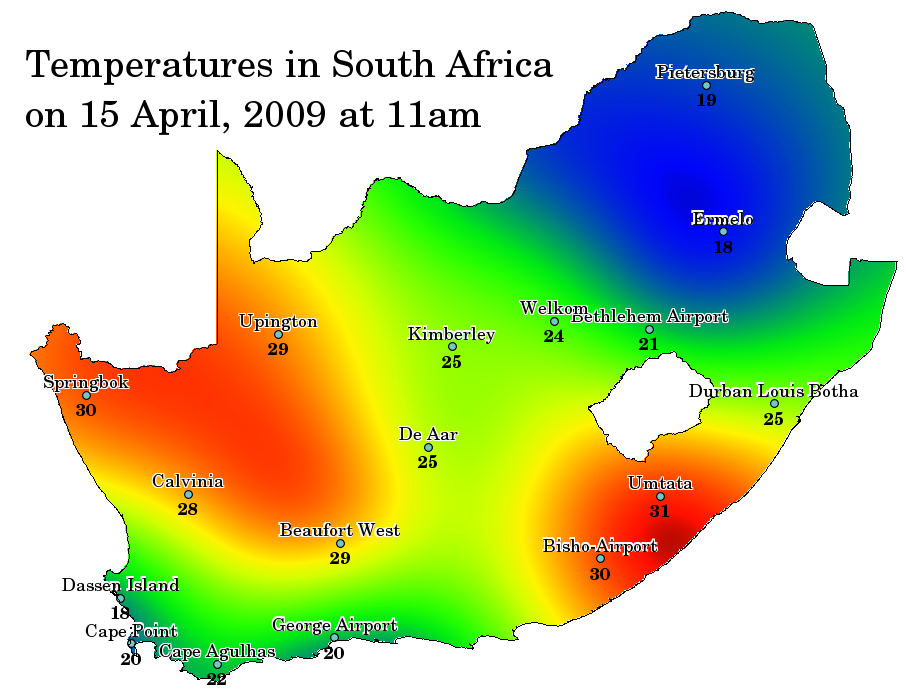
\includegraphics[clip=true, width=0.5\textwidth]{temperatures_20090415}
\end{center}
\end{figure}

\textbf{Spatial interpolation} is the process of using points with known values to
estimate values at other unknown points. For example, to make a precipitation
(rainfall) map for your country, you will not find enough evenly spread
weather stations to cover the entire region. Spatial interpolation can
estimate the temperatures at locations without recorded data by using known
temperature readings at nearby weather stations (see Figure
\ref{fig:temperature}). This type of interpolated surface is often called a
\textbf{statistical surface}.
Elevation data, precipitation, snow accumulation, water table and population
density are other types of data that can be computed using interpolation.

Because of high cost and limited resources, data collection is usually
conducted only in a limited number of selected point locations. In GIS,
spatial interpolation of these points can be applied to create a raster
surface with estimates made for all raster cells. 

In order to generate a continuous map, for example, a digital elevation map
from elevation points measured with a GPS device, a suitable interpolation
method has to be used to optimally estimate the values at those locations
where no samples or measurements were taken. The results of the interpolation
analysis can then be used for analyses that cover the whole area and for
modelling. 

There are many interpolation methods. In this introduction we will present
two widely used interpolation methods called \textbf{Inverse Distance
Weighting} (IDW) and \textbf{Triangulated Irregular Networks (TIN)}. If you
are looking for additional
interpolation methods, please refer to the further reading section at the end
of this topic. 

\subsection{Inverse Distance Weighted (IDW)}

In the IDW interpolation method, the sample points are weighted during
interpolation such that the influence of one point relative to another
declines with distance from the unknown point you want to create (see
Figure \ref{fig:idw}). 

\begin{figure}[ht]
   \begin{center}
   \caption{Inverse Distance Weighted interpolation based on weighted sample
point distance (left). Interpolated IDW surface from elevation vector points
(right). Image Source: Mitas, L., Mitasova, H. (1999).}
\label{fig:idw}\smallskip
   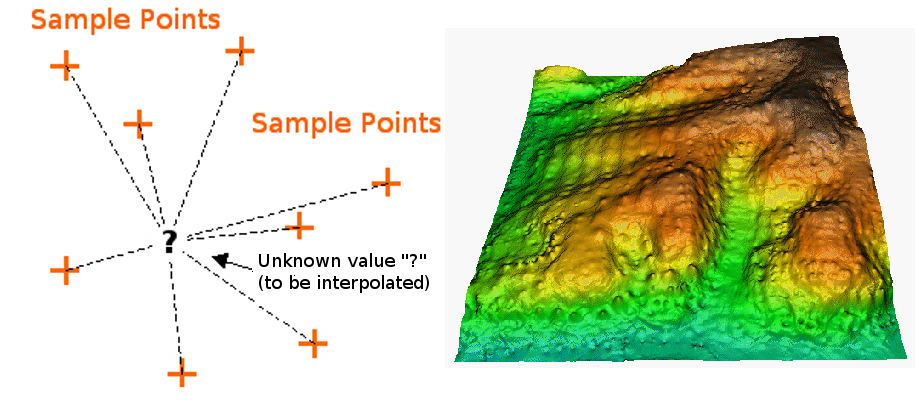
\includegraphics[clip=true, width=0.6\textwidth]{interpolation_IDW}
\end{center}
\end{figure}

Weighting is assigned to sample points through the use of a weighting
coefficient that controls how the weighting influence will drop off as the
distance from new point increases. The greater the weighting coefficient, the
less the effect points will have if they are far from the unknown point
during the interpolation process. As the coefficient increases, the value of
the unknown point approaches the value of the nearest observational point. 

It is important to notice that the IDW interpolation method also has some
disadvantages: The quality of the interpolation result can decrease, if the
distribution of sample data points is uneven. Furthermore, maximum and
minimum values in the interpolated surface can only occur at sample data
points. This often results in small peaks and pits around the sample data
points as shown in Figure \ref{fig:idw}.

In GIS, interpolation results are usually shown as a 2 dimensional raster
layer. In Figure \ref{fig:qgisidw}, you can see a typical IDW interpolation
result, based on elevation sample points collected in the field with a GPS
device.

\begin{figure}[ht]
   \begin{center}
   \caption{IDW interpolation result from irregularly collected elevation
sample points (shown as black crosses).}
\label{fig:qgisidw}\smallskip
   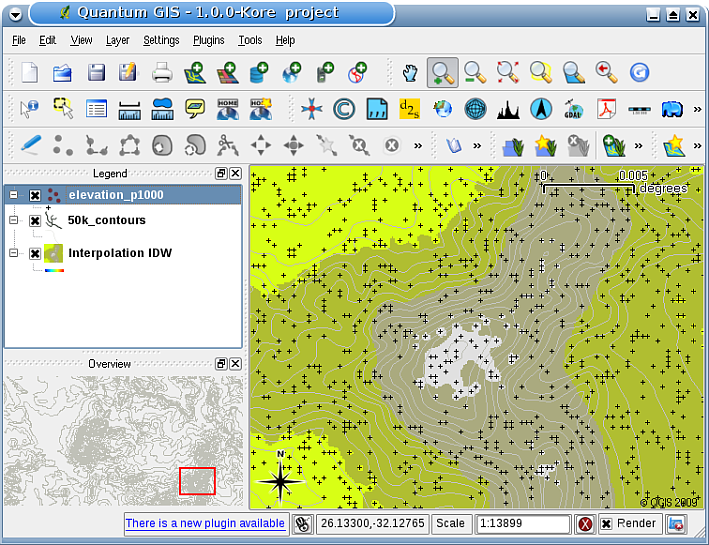
\includegraphics[clip=true, width=0.6\textwidth]{qgis_interpolation_IDW}
\end{center}
\end{figure}

\subsection{Triangulated Irregular Network (TIN)}

TIN interpolation is another popular tool in GIS. A common TIN algorithm is
called \textbf{Delaunay} triangulation. It tries to create a surface formed by
triangles of nearest neighbour points. To do this, circumcircles around
selected sample points are created and their intersections are connected to a
network of non overlapping and as compact as possible triangles (see Figure
\ref{fig:tin}).

%% Minipage to put both figures on one page
\begin{figure}[htpb]
   \begin{minipage}[h]{\textwidth}
   \begin{center}
   \caption{Delaunay triangulation with circumcircles around the red sample
data. The resulting interpolated TIN surface created from elevation vector
points is shown on the right. Image Source: Mitas, L., Mitasova, H. (1999).}
   \label{fig:tin}\smallskip
   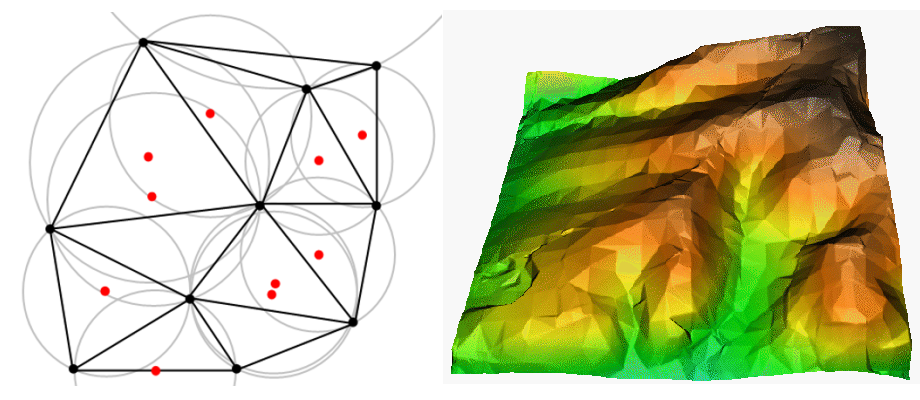
\includegraphics[clip=true, width=0.8\textwidth]{interpolation_TIN}
   \end{center}
   \end{minipage} \\
   \vspace{1cm}
   \begin{minipage}[h]{\textwidth}
   \begin{center}
   \caption{Delaunay TIN interpolation result from irregularly collected
rainfall sample points (blue circles).}
   \label{fig:qgistin}\smallskip
   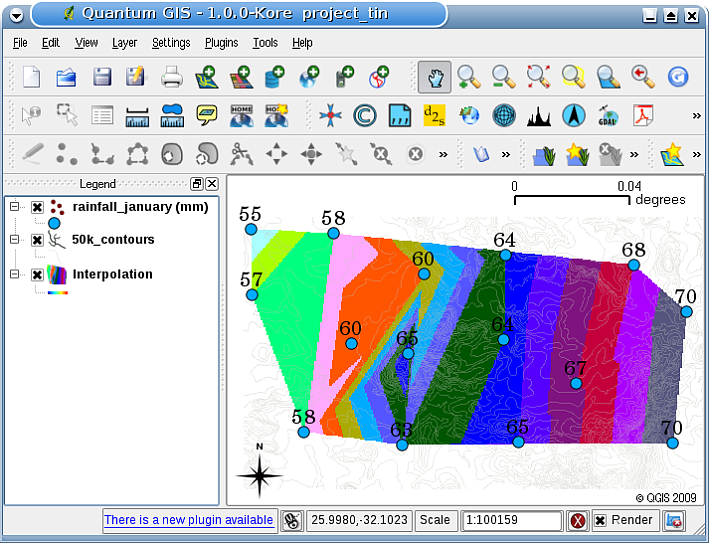
\includegraphics[clip=true, width=0.8\textwidth]{qgis_interpolation_TIN}
   \end{center}
   \end{minipage}
\end{figure}

The main disadvantage of the TIN interpolation is that the surfaces are not
smooth and may give a jagged appearance. This is caused by discontinuous
slopes at the triangle edges and sample data points. In addition,
triangulation is generally not suitable for extrapolation beyond the area
with collected sample data points (see Figure \ref{fig:qgistin}).

\subsection{Common problems / things to be aware of}

It is important to remember that there is no single interpolation method that
can be applied to all situations. Some are more exact and useful than others
but take longer to calculate. They all have advantages and disadvantages. In
practice, selection of a particular interpolation method should depend upon
the sample data, the type of surfaces to be generated and tolerance of
estimation errors. Generally, a three step procedure is recommended:

\begin{enumerate}
\item Evaluate the sample data. Do this to get an idea on how data are
distributed in the area, as this may provide hints on which interpolation
method to use. 
\item Apply an interpolation method which is most suitable to both the sample
data and the study objectives. When you are in doubt, try several methods, if
available. 
\item Compare the results and find the best result and the most suitable method.
This may look like a time consuming process at the beginning. However, as you
gain experience and knowledge of different interpolation methods, the time
required for generating the most suitable surface will be greatly reduced. 
\end{enumerate}

\subsection{Other interpolation methods}

Although we concentrated on IDW and TIN interpolation methods in this
worksheet, there are more spatial interpolation methods provided in GIS, such
as Regularized Splines with Tension (RST), Kriging or Trend Surface
interpolation. See the additional reading section below for a web link. 

\subsection{What have we learned?}

Let's wrap up what we covered in this worksheet:

\begin{itemize}
\item \textbf{Interpolation} uses vector points with known values to estimate
values at unknown locations to create a raster surface covering an entire area.
\item The interpolation result is typically a \textbf{raster} layer.
\item It is important to \textbf{find a suitable interpolation method} to
optimally estimate values for unknown locations.
\item \textbf{IDW interpolation} gives weights to sample points, such that
the influence of one point on another declines with distance from the new
point being estimated.
\item \textbf{TIN interpolation} uses sample points to create a surface
formed by triangles based on nearest neighbour point information.
\end{itemize}

\subsection{Now you try!}

Here are some ideas for you to try with your learners:

\begin{itemize}
\item The Department of Agriculture plans to cultivate new land in your area but
apart from the character of the soils, they want to know if the rainfall is
sufficient for a good harvest. All the information they have available comes
from a few weather stations around the area. Create an interpolated surface
with your learners that shows which areas are likely to receive the highest
rainfall.
\item The tourist office wants to publish information about the weather conditions
in January and February. They have temperature, rainfall and wind strength
data and ask you to interpolate their data to estimate places where tourists
will probably have optimal weather conditions with mild temperatures, no
rainfall and little wind strength. Can you identify the areas in your region
that meet these criteria?
\end{itemize}

\subsection{Something to think about}

If you don't have a computer available, you can use a toposheet and a ruler
to estimate elevation values between contour lines or rainfall values between
fictional weather stations. For example, if rainfall at weather station A is
50 mm per month and at weather station B it is 90 mm, you can estimate, that
the rainfall at half the distance between weather station A and B is 70 mm.

\subsection{Further reading}

\textbf{Books}: 

\begin{itemize}
\item Chang, Kang-Tsung (2006): Introduction to Geographic Information Systems. 3rd
Edition.  McGraw Hill. (ISBN 0070658986)
\item DeMers, Michael N. (2005): Fundamentals of Geographic Information Systems.
3rd Edition. Wiley. (ISBN 9814126195)
\item Mitas, L., Mitasova, H. (1999): Spatial Interpolation. In: P.Longley, M.F.
Goodchild, D.J. Maguire, D.W.Rhind (Eds.), Geographical Information Systems:
Principles, Techniques, Management and Applications, Wiley. 
\end{itemize}

\textbf{Websites}:
 
\url{http://en.wikipedia.org/wiki/Interpolation} \\
\url{http://en.wikipedia.org/wiki/Delaunay\_triangulation} \\
\url{http://www.agt.bme.hu/public_e/funcint/funcint.html}

The QGIS User Guide also has more detailed information on interpolation tools
provided in QGIS.

\subsection{What's next?}

This is the final worksheet in this series. We encourage you to explore QGIS
and use the QGIS manual to discover all the other things you can
do with GIS software!


